\section{Exercise 7.4 Play with subgradient optimization}
\textbf{Problem:} Play with the MATLAB code for Subgradient Optimization. Try bigger examples. Try different ideas for the step size. Also, Theorem 7.5, together with the fact that Subgradient Optimization converges in the limit to a a solution of the Lagrangian Dual together, tells us that the y and π produced should be optimal for the dual of (\ref{eq: probq}). Check this out: see to what extent $y$ and $\pi$ are feasible for the dual of (\ref{eq: probq}) once the lower bounds on $z$ are good.
\begin{equation}
\label{eq: probq}
  \begin{array}{lrcll}
    z:=\min
    & \multicolumn{4}{l}{c'x} \\
    \text{s.t.}
    & Ex=h;\\
    & Ax=b;\\
    & x\geq0.
  \end{array}
\end{equation}

\textbf{Solution:} 

Using hte MATLAB code for Subgradient Optimization, we generate Figure \ref{fig: ex7_4_k} with $\lambda_k=\frac{1}{k}$, $n=50$, $m_1=15$, $m_2=10$, the default values. In the figure, the value $v(\widehat{y})$, which is referred as Lagrangian lower bound, converges and becomes stable around $k=40$.
 
\begin{figure}[h]
\centering
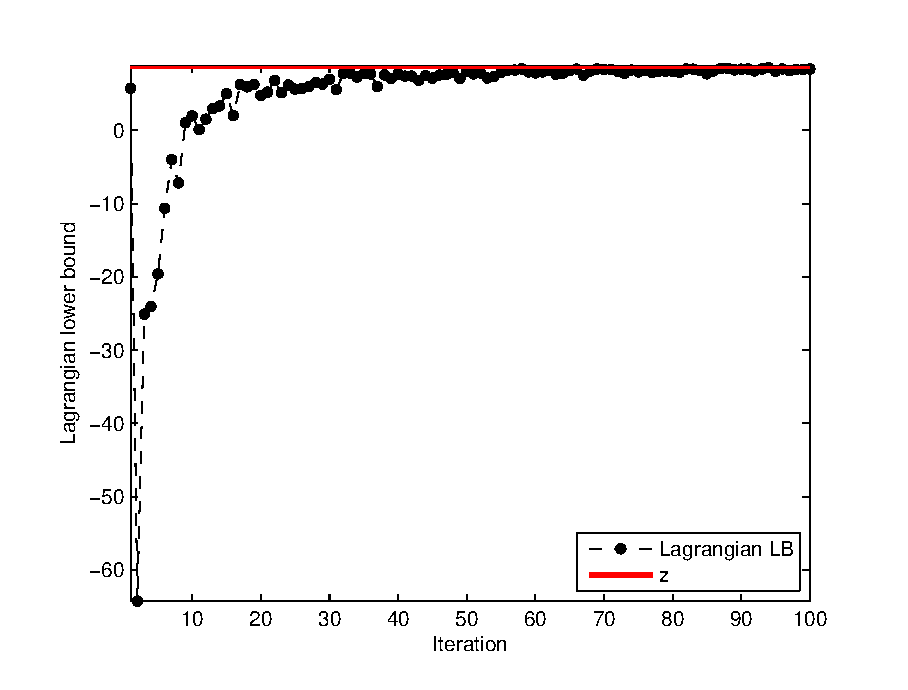
\includegraphics[width=3.0in]{./p4/ex7_4_k}
\captionof{figure}{Subgradient Optimization with $\lambda_k=\frac{1}{k}$, $n=50$, $m_1=15$, $m_2=10$.}
\label{fig: ex7_4_k}
\end{figure}

We first try bigger examples. We vary $n$ from 50 to 100 and 100, which are shown in Figure \ref{fig: ex7_4_k_n100} and Figure \ref{fig: ex7_4_k_n1000}. Compared to  Figure \ref{fig: ex7_4_k},  convergence with $n=100$ becomes stable around $k=20$, which is more earlier than smaller $n$. Also $v(\widehat{y})$ is more stable after $n=20$. On the other hand, a much larger problem with $n=1000$ is much less stable than $n=50$ and $n=100$, indicating that larger variable number may have negative impact on the convergence.  

\begin{figure}[!ht]
\centering
\begin{minipage}{0.49\textwidth}
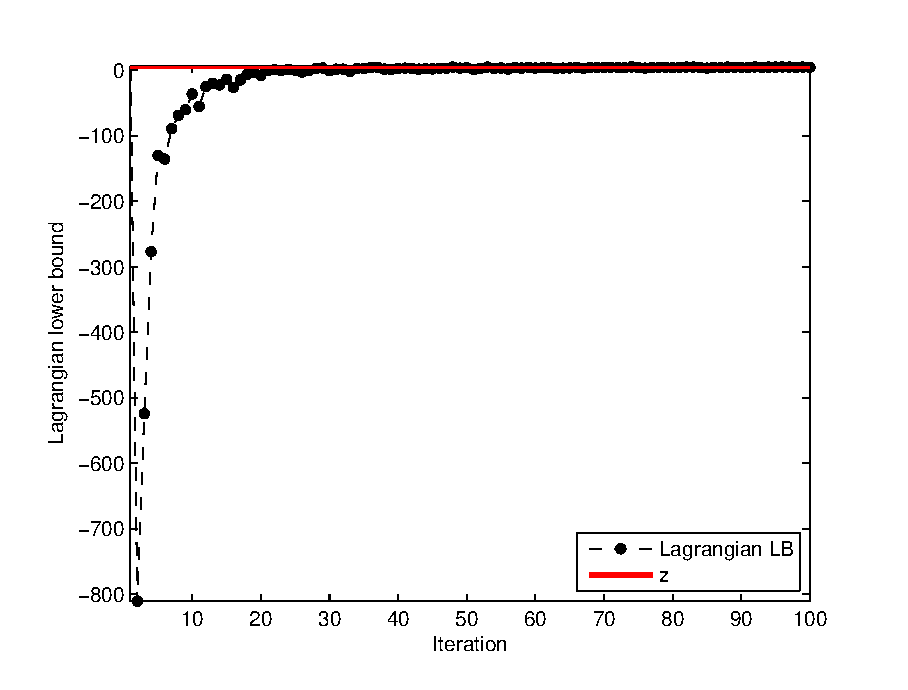
\includegraphics[width=3.0in]{./p4/ex7_4_k_n100}
\captionof{figure}{Subgradient Optimization with $\lambda_k=\frac{1}{k}$, $n=100$, $m_1=15$, $m_2=10$.}
\label{fig: ex7_4_k_n100}
\end{minipage}
\begin{minipage}{0.49\textwidth}
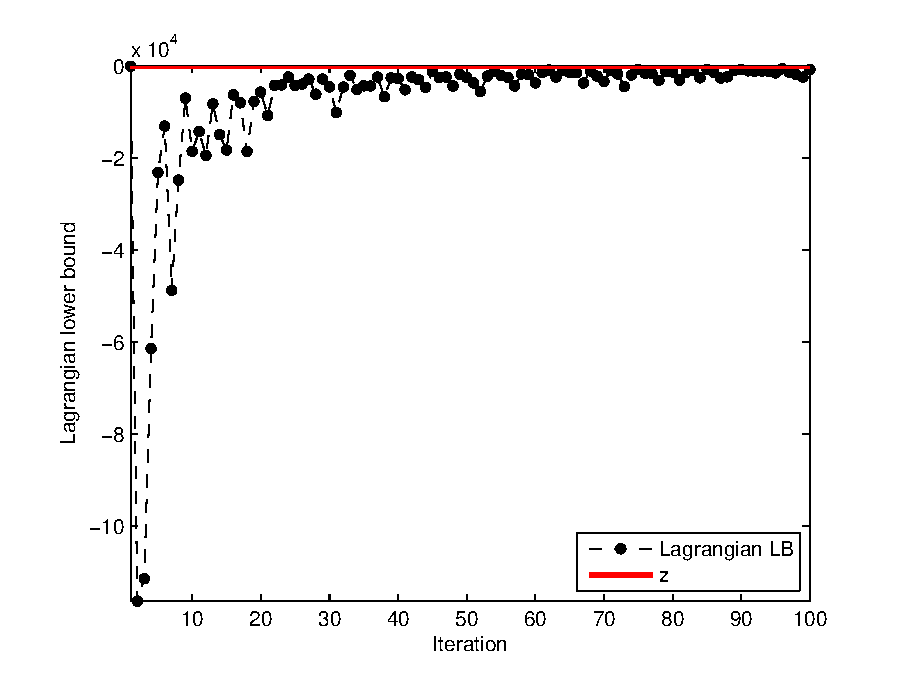
\includegraphics[width=3.0in]{./p4/ex7_4_k_n1000}
\captionof{figure}{Subgradient Optimization with $\lambda_k=\frac{1}{k}$, $n=1000$,  $m_1=15$, $m_2=10$.}
\label{fig: ex7_4_k_n1000}
\end{minipage}
\end{figure}

We then vary $m_1$, the column number of $E$ in (\ref{eq: probq}), from 15 to 25 and 35, which are shown in Figure \ref{fig: ex7_4_k_m1_25} and Figure \ref{fig: ex7_4_k_m1_35}. Compared to  Figure \ref{fig: ex7_4_k},  both cases converge slower than the one with $m_1=15$. But interestingly, the situation is not strictly getting worse when $m_1$ increase, as we can see that $m_1=25$ converges slower than larger $m_1$.

\begin{figure}[!ht]
\centering
\begin{minipage}{0.49\textwidth}
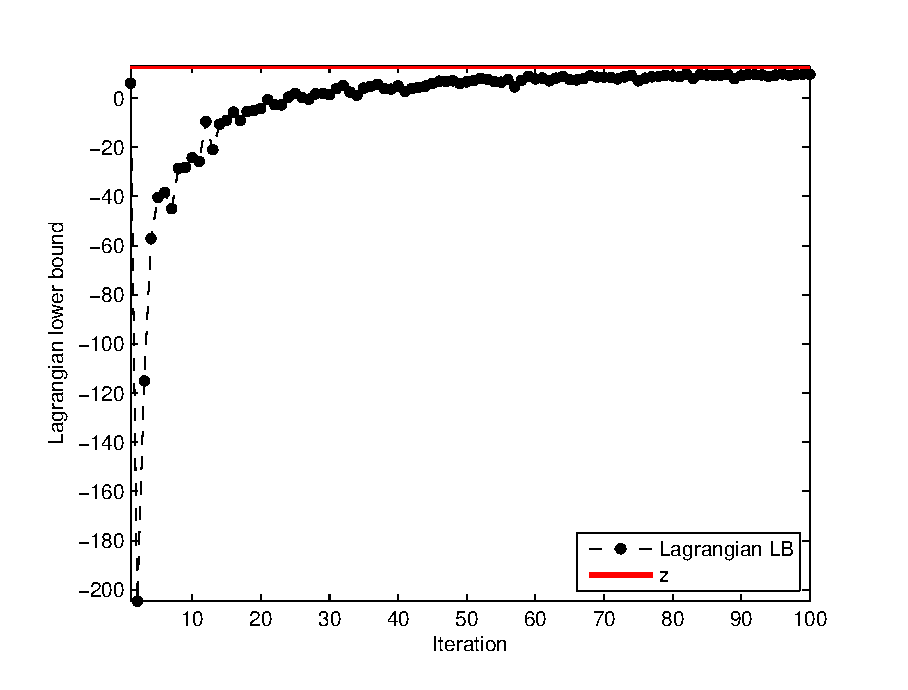
\includegraphics[width=3.0in]{./p4/ex7_4_k_m1_25}
\captionof{figure}{Subgradient Optimization with $\lambda_k=\frac{1}{k}$, $n=50$, $m_1=25$, $m_2=10$.}
\label{fig: ex7_4_k_m1_25}
\end{minipage}
\begin{minipage}{0.49\textwidth}
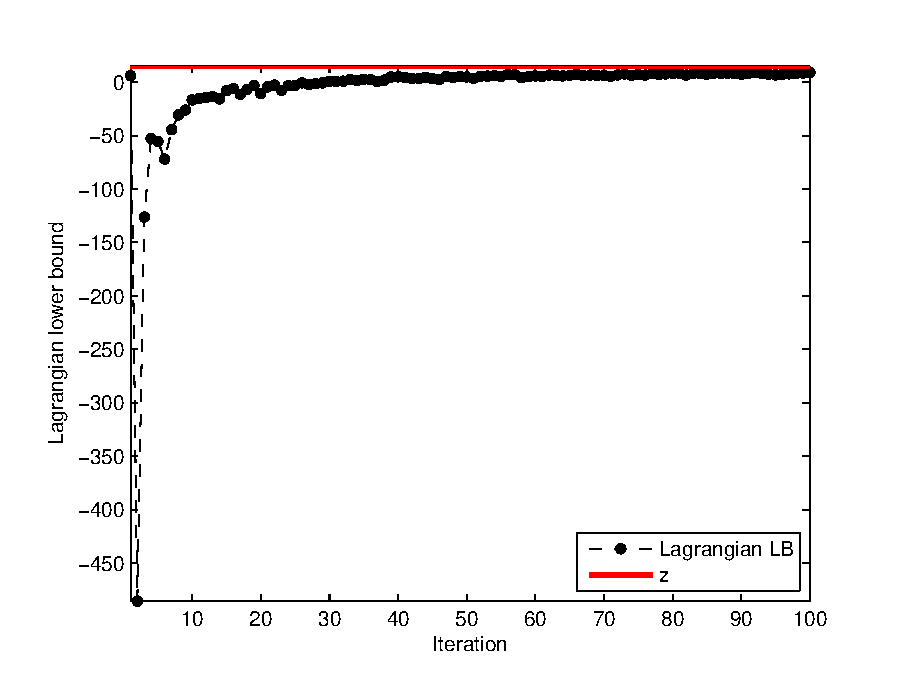
\includegraphics[width=3.0in]{./p4/ex7_4_k_m1_35}
\captionof{figure}{Subgradient Optimization with $\lambda_k=\frac{1}{k}$, $n=50$, $m_1=35$, $m_2=10$.}
\label{fig: ex7_4_k_m1_35}
\end{minipage}
\end{figure}

After that, we vary $m_2$, the column number of $A$ in (\ref{eq: probq}), from 10 to 20 and 30, which are shown in Figure \ref{fig: ex7_4_k_m2_20} and Figure \ref{fig: ex7_4_k_m2_30}. Figure \ref{fig: ex7_4_k_m2_20} with $m_2=20$ is quite similar to Figure \ref{fig: ex7_4_k} with $m_2=10$, while Figure \ref{fig: ex7_4_k_m2_30} with $m_2=30$ is slightly worse compared to them.

\begin{figure}[!ht]
\centering
\begin{minipage}{0.49\textwidth}
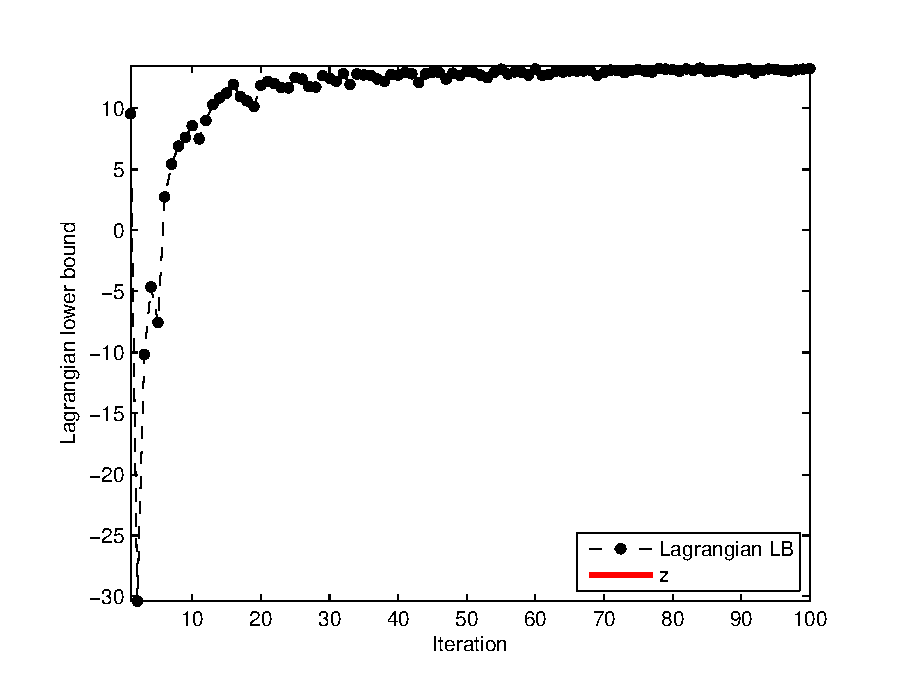
\includegraphics[width=3.0in]{./p4/ex7_4_k_m2_20}
\captionof{figure}{Subgradient Optimization with $\lambda_k=\frac{1}{k}$, $n=50$, $m_1=15$, $m_2=20$.}
\label{fig: ex7_4_k_m2_20}
\end{minipage}
\begin{minipage}{0.49\textwidth}
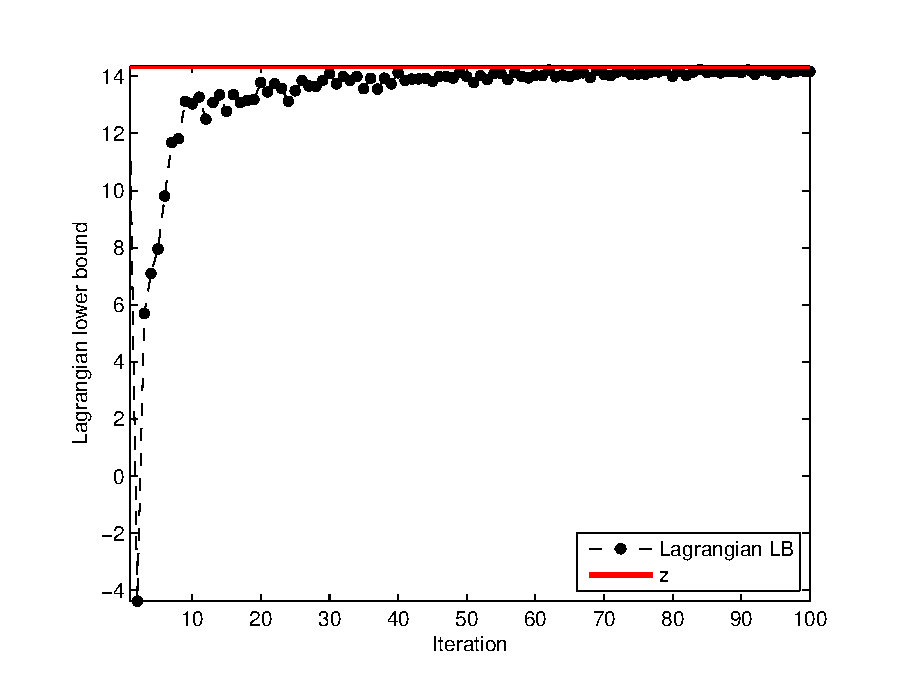
\includegraphics[width=3.0in]{./p4/ex7_4_k_m2_30}
\captionof{figure}{Subgradient Optimization with $\lambda_k=\frac{1}{k}$, $n=50$, $m_1=15$, $m_2=30$.}
\label{fig: ex7_4_k_m2_30}
\end{minipage}
\end{figure}

For the experiments of varying $n$, $m_1$, $m_2$ above, $v(\widehat{y})$ generally converges between $k=50$ to $k=100$.

Next, we try some other ideas of choosing the step size $\lambda_k$. For these ideas, we need to make sure that property $\sum_{k=1}^{\infty} \lambda^2_k < +\infty$, and $\sum_{k=1}^{\infty} \lambda_k = +\infty$ are satisfied. First we choose $\lambda_k=\frac{1}{2k}$ and $\lambda_k=\frac{1}{2k+1}$, which satisfy the properties in the same way of $\lambda_k=\frac{1}{k}$. Figure \ref{fig: ex7_4_2k} and Figure \ref{fig: ex7_4_2k1} shows the result. Besides these two, we also try $\lambda_k=\frac{1}{(k+1)log(k+1)}$, and the result is shown in Figure \ref{fig: ex7_4_klogk}. For this one, it is easy to see that $\sum_{k=1}^{\infty} \lambda^2_k < +\infty$ is satisfied since $\sum_{k=1}^{\infty} (\frac{1}{k+1})^2 < +\infty$ and the increasing speed of $\frac{1}{k+1}$ is faster than $\frac{1}{log(k+1)}$. At the same time, $\lambda_k=\frac{1}{2k+1}$ property is also satisfied since $\int \frac{1}{kln(k)} dk=ln(ln(k))+C$, which is unbounded.

\begin{figure}[!ht]
\centering
\begin{minipage}{0.49\textwidth}
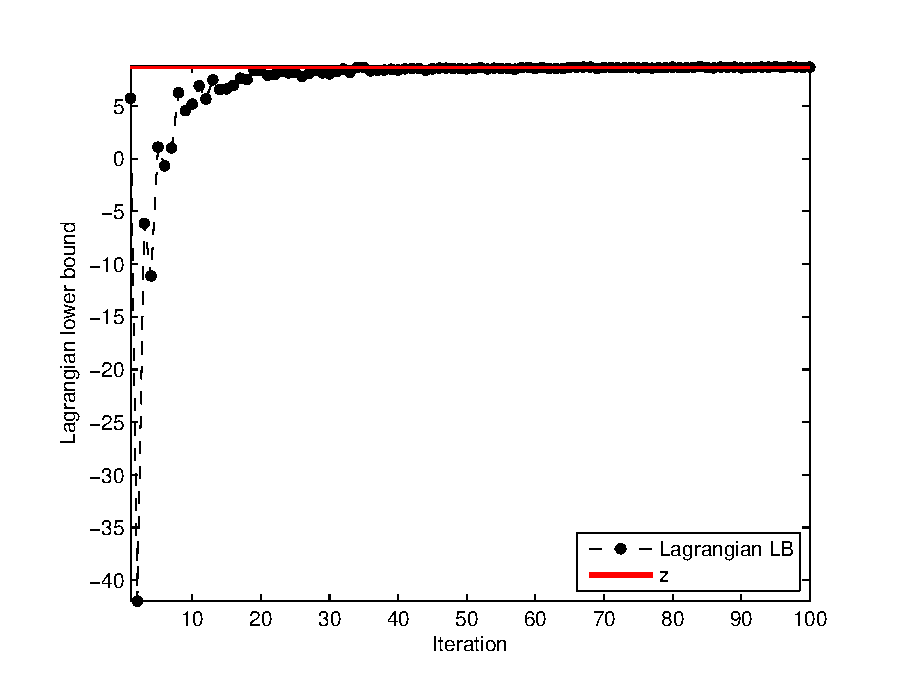
\includegraphics[width=3.0in]{./p4/ex7_4_klogk}
\captionof{figure}{Subgradient Optimization with $\lambda_k=\frac{1}{(k+1)log(k+1)}$, $n=50$, $m_1=15$, $m_2=10$.}
\label{fig: ex7_4_klogk}
\end{minipage}
\end{figure}

\begin{figure}[!ht]
\centering
\begin{minipage}{0.49\textwidth}
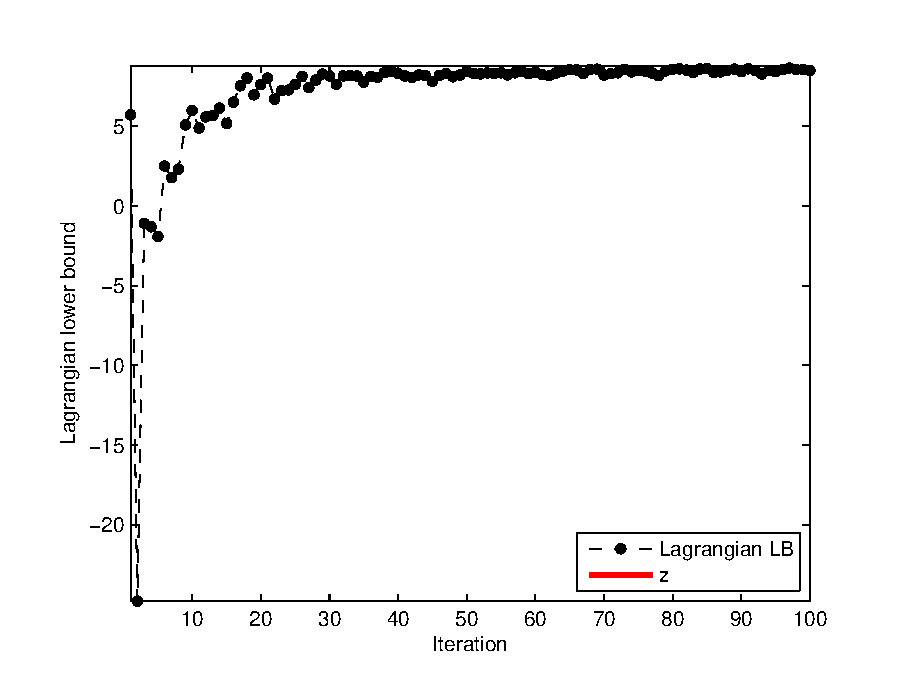
\includegraphics[width=3.0in]{./p4/ex7_4_2k}
\captionof{figure}{Subgradient Optimization with $\lambda_k=\frac{1}{2k}$, $n=50$, $m_1=15$, $m_2=30$.}
\label{fig: ex7_4_2k}
\end{minipage}
\begin{minipage}{0.49\textwidth}
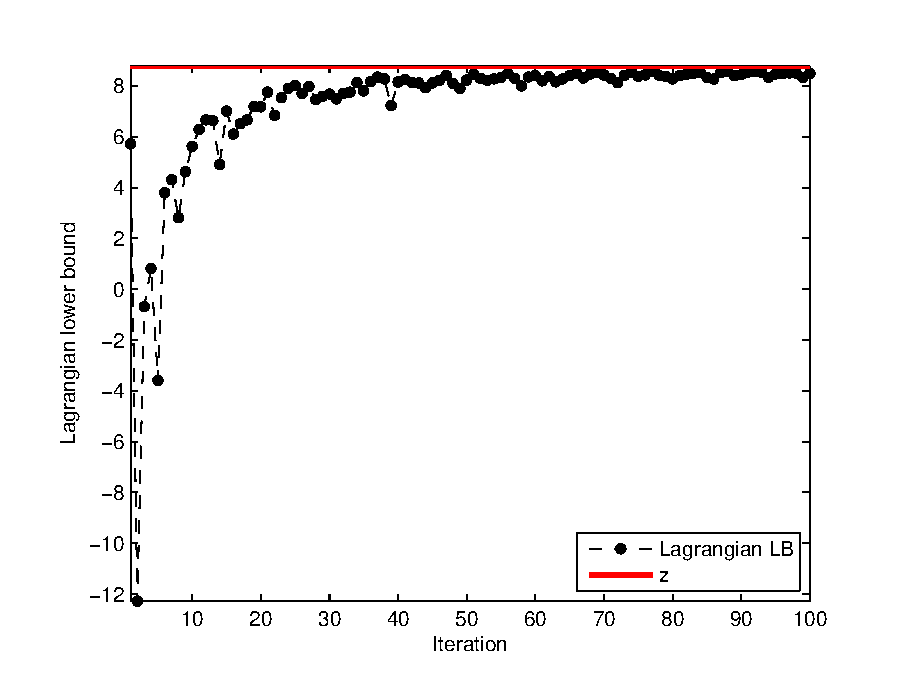
\includegraphics[width=3.0in]{./p4/ex7_4_2k1}
\captionof{figure}{Subgradient Optimization with $\lambda_k=\frac{1}{2k+1}$, $n=50$, $m_1=15$, $m_2=10$.}
\label{fig: ex7_4_2k1}
\end{minipage}
\end{figure}

Compare Figure \ref{fig: ex7_4_k}, Figure \ref{fig: ex7_4_2k}, Figure \ref{fig: ex7_4_2k1}, and Figure \ref{fig: ex7_4_klogk}, we can see that $\lambda_k=\frac{1}{k}$ performs similar to $\lambda_k=\frac{1}{2k}$,  while $\lambda_k=\frac{1}{2k+1}$ converges the slowest and is the most unstable one. Among them, $\lambda_k=\frac{1}{(k+1)log(k+1)}$ performs the best, showing a good property of accelerating the convergence.

\begin{table}[!ht]
\centering
\begin{tabular}{|c|c|c|c|c|}
\hline
$\lambda_k$ & $n$ & $m_1$  & $m_2$ & Dual infeasibility rate \\
\hline
$\frac{1}{k}$  & 50 & 15  & 10 & 0.1839 \\
\hline
$\frac{1}{k}$  & 100 & 15  & 10 & 2.1201 \\
\hline
$\frac{1}{k}$  & 1000 & 15  & 10 & 136.5 \\
\hline
$\frac{1}{k}$  & 50 & 25  & 10 & 0 \\
\hline
$\frac{1}{k}$  & 50 & 35  & 10 & 0.3204 \\
\hline
$\frac{1}{k}$  & 50 & 15  & 20 & 0.0523 \\
\hline
$\frac{1}{k}$  & 50 & 15  & 30 & 0.1068 \\
\hline
$\frac{1}{2k}$  & 50 & 15  & 10 & 0.1847 \\
\hline
$\frac{1}{2k+1}$  & 50 & 15  & 10 & 0.0021 \\
\hline
$\frac{1}{(k+1)log(k+1)}$  & 50 & 15  & 10 & 0.0209 \\
\hline
\end{tabular}
\caption{Dual infeasibility rate under different conditions}
\label{tab: dual_feasible}
\end{table}

At last, we evaluate how feasible are the $\widehat{y}$ and $\widehat{\pi}$ after solving the Lagrangian dual. From the Subgradient Optimization process we can get $\widehat{y}$, and from MATLAB function \texttt{linprog()} we can get the dual solution $\widehat{\pi}$. For  $\widehat{y}$ and $\widehat{\pi}$ to be feasible, we need to have $\widehat{y}'E+\widehat{\pi}'A \geq c'$, so we calculate $d=c'- (\widehat{y}'E+\widehat{\pi}'A)$, and calculate dual infeasibility rate as $\sum_{d_i < 0} d_i^2 $. The higher the rate, more feasible are $\widehat{y}$ and $\widehat{\pi}$. 

Table \ref{tab: dual_feasible} shows the dual infeasibility rates with different $\lambda_k$, $n$, $m_1$, and $m_2$. From the table, $\widehat{y}$ and $\widehat{\pi}$ are more feasible when the problem becomes larger.